Der Fotoeffekt ist der heutige Name für den Hallwachseffekt und die Erforschung und Mathematisierung erfolgte von Max Planck und Albert Einstein Anfang des 20. Jahrhunderts.

Nun war qualitativ bekannt, dass Licht ab einer bestimmten Wellenlänge Elektronen aus Metall auslöst, allerdings gab es weder eine quantitative Bestimmung der Menge dieser Elektronen, noch eine Gleichung zur Bestimmung der Strahlungsenergie.

\begin{NiceToKnow}
	Qualitative Bestimmung heißt, man kann das Ergebnis eines Versuches so vorhersagen, dass man zwar den Effekt kennt und Aussagen über Dinge wie Richtung einer möglichen Bewegung, etc. machen kann, aber keine exakten Werte angeben kann.
	
	Mit einer quantitativen Aussage gibt man auch exakte Werte an.
\end{NiceToKnow}


\subsection{Fotozelle}

Bei dem Experiment kommt die sogenannte Fotozelle zum Einsatz.

Eine Fotozelle ist ein evakuierter (im Inneren ist ein Vakuum) Glaszylinder, in welchem sich, im gröbsten Sinne, ein Kondensator befindet. An zwei Elektroden die sich im Inneren befinden, eine ist ringförmig und die andere halbkugelförmig, lassen sich Messgeräte und Spannungsquellen anschließen.
%Cue for pic

\subsection{Aufbau und Durchführung}

Eine Fotozelle wird mit UV-Licht bestrahlt, dadurch werden Elektronen Elektronen aus der schalenförmigen Kathode aus Natrium (ein Metall) ausgelöst. 

Es kann beobachtet werden, dass ein (wenn auch extrem kleiner) Strom fließt, wenn man die beiden Elektronen über einen Widerstand und ein Strommessgerät verbindet.

Eine Gegenspannung $U_{max}$ wird an der Fotozelle angelegt und so lange erhöht, bis kein Strom $I$ mehr gemessen wird.


\subsection{Deutung}

Einige der herausgeschlagenen Elektronen treffen auf der ringförmigen Anode auf; dies erzeugt den Strom der gemessen wird.

Diese Elektronen besitzen eine demnach eine kinetische Energie $E_{kin}$ (Siehe: \referenz{subsec:Energieformen}), wenn sie ausgelöst werden. Durch die Gegenspannung müssen sie gegen ein entgegengesetztes elektrisches Feld "ankämpfen" (Siehe: \referenz{sec:ElektronenwegungImEFeld}). Wenn kein Strom $I$ mehr gemessen wird ist die elektrische Energie $E_{el} = U \cdot e$ (Siehe: \gleichungsreferenz{eq:arbeit_kondensator} mit der Feldstärke $E$ (nicht verwechseln mit der Energie, beides hat das Formelzeichen $E$) im Kondensator $E=\frac{U}{d}$) gleich der kinetischen Energie $E_{kin} = \frac{1}{2} m v^2$ (Siehe: \gleichungsreferenz{eq:ekin}):

\begin{align}
\begin{split}
	E_{el} &= E_{kin} \\
\end{split}
\end{align}


\subsection{Photonenenergie}

Nun kann man davon ausgehen, dass die Energie \emph{eines} Lichtphotons gleich der kinetischen Energie \emph{eines} ausgelösten Elektrons ist. Da es, durch andere Faktoren, Unterschiede in den Geschwindigkeiten der herausgeschlagenen Elektronen gibt, werden nur die schnellsten, also die energiereichsten Elektronen in Betracht gezogen. 

Es gibt allerdings eine gewisse Austrittsarbeit $W_A$, abhängig von dem Material der Kathode, die notwendig ist, um ein Elektron überhaupt aus der Platte zu lösen, ohne im dabei eine kinetische Energie mitzugeben. Daher muss diese Größe von der Photonenenergie $E_{phot}$ abgezogen werden.

Ferner ist $E_{kin}$, wie gerade gezeigt, gleich $E_{el}$, sodass man schreiben kann:

\begin{align} \label{eq:EelmitWA}
\begin{split}
	E_{el} &= E_{phot} - W_A \\
\end{split}
\end{align}

\begin{figure}[h!]
	\centering
	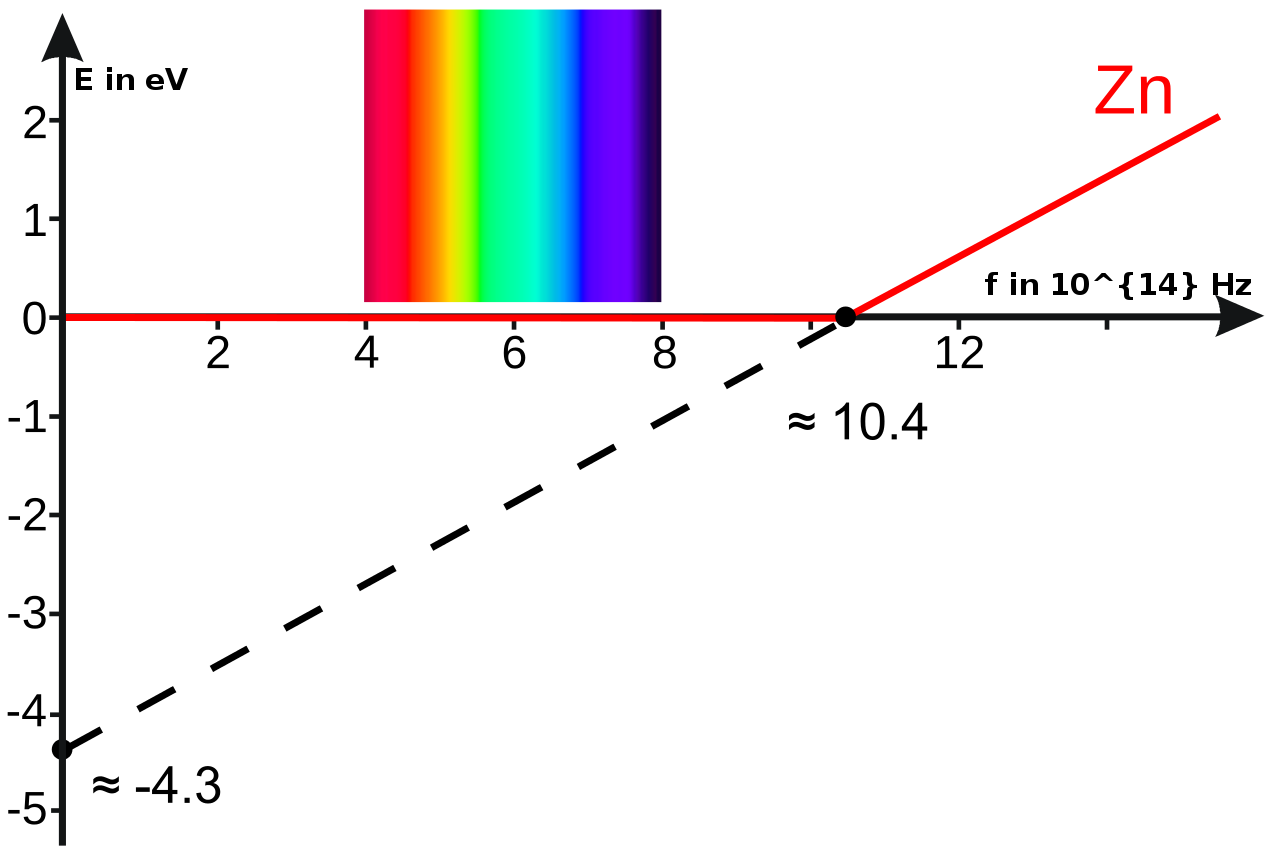
\includegraphics[width=0.7\textwidth]{PhotoelektischerEffekt}
	\caption{Aufführung der Energie der Elektronen (in Elektronenvolt: $1 eV = q_e J \approx 1,602 J$) über der Frequenz des Lichtes. Ein Spektrum gibt eine Referenz des Bereiches.}
	\label{fig:Fotoeffekt}
\end{figure}

Aus der Abbildung \ref{fig:Fotoeffekt}\endnote{\glqq Photoelectric effect diagram no label\grqq{} by Klaus-Dieter Keller - File:Photoelectric effect diagram.svg. Licensed under CC BY 3.0 via Wikimedia Commons. Modified by Till Blaha (Labeling) - \url{https://commons.wikimedia.org/wiki/File:Photoelectric_effect_diagram_no_label.svg}} ist ein linearer Anstieg der Photonenenergie ersichtlich. Max Planck folgerte daraus, dass es ein Naturkonstante gibt, die die Steigung definiert.

Einstein formulierte dann die, sehr wichtige, Einstein'sche Gleichung:

\begin{align}	\label{eq:einsteinscheGleichung}
\begin{split}
	E_{phot} = h \cdot f
\end{split}
\end{align}

\noindent Hierbei ist $h$ das \glqq Plank'sche Wirkungsquantum\grqq , eine Naturkonstante (\casio{06}), mit:

\begin{equation}
	h \approx 6,626 \cdot 10^{-34} Js = 6,626 \cdot 10^{-34} \frac{kg \cdot m^2}{s}
\end{equation}


\subsection{Austrittsarbeit}

Mit Gleichung \ref{eq:einsteinscheGleichung} kann man die Gleichung \ref{eq:EelmitWA} weiter auflösen und erhält für $W_A$:

\begin{align} \label{eq:Austrittsarbeit}
\begin{split}
	E_{el} &= h \cdot f - W_A \\
	e \cdot U &= h \cdot f - W_A \\
	W_A &= h \cdot f - e \cdot U
\end{split}
\end{align}


\subsection{Grenzfrequenz}

Für die Grenzfrequenz $f_{gr}$, also die Frequenz, die das Licht mindestens haben muss, um Elektronen aus einem bestimmten Material zu lösen, lässt sich aus Gleichung \ref{eq:EelmitWA} ableiten, wenn man $E{el} = 0$ setzt:

\begin{align} \label{eq:Grenzfrequenz}
\begin{split}
	0 &= E_{phot,gr} - W_A \\
	W_A &= E_{phot,gr} \\
	W_A &= h \cdot f_{gr} \\
	f_{gr} &= \frac{W_A}{h}
\end{split}
\end{align}


